\newbool{showpfp}

\newcommand{\cvheader}[1]{
  \begin{center}
    \begin{tabularx}{\textwidth} { 
        >{\raggedright\arraybackslash}X 
      >{\raggedleft\arraybackslash}X  }
      \huge Markus A.G. Amano & #1\\
      \hline
      Website: \url{https://markuspad.com/}& 
      GitHub: \href{https://github.com/inokawazu}{inokawazu}\\
      Email: markus.a.amano[at]gmail.com & \href{https://inspirehep.net/authors/1778034}{iNSPIREHEP}\\
      Nationality: USA & \\
                       & \ifbool{showpfp}{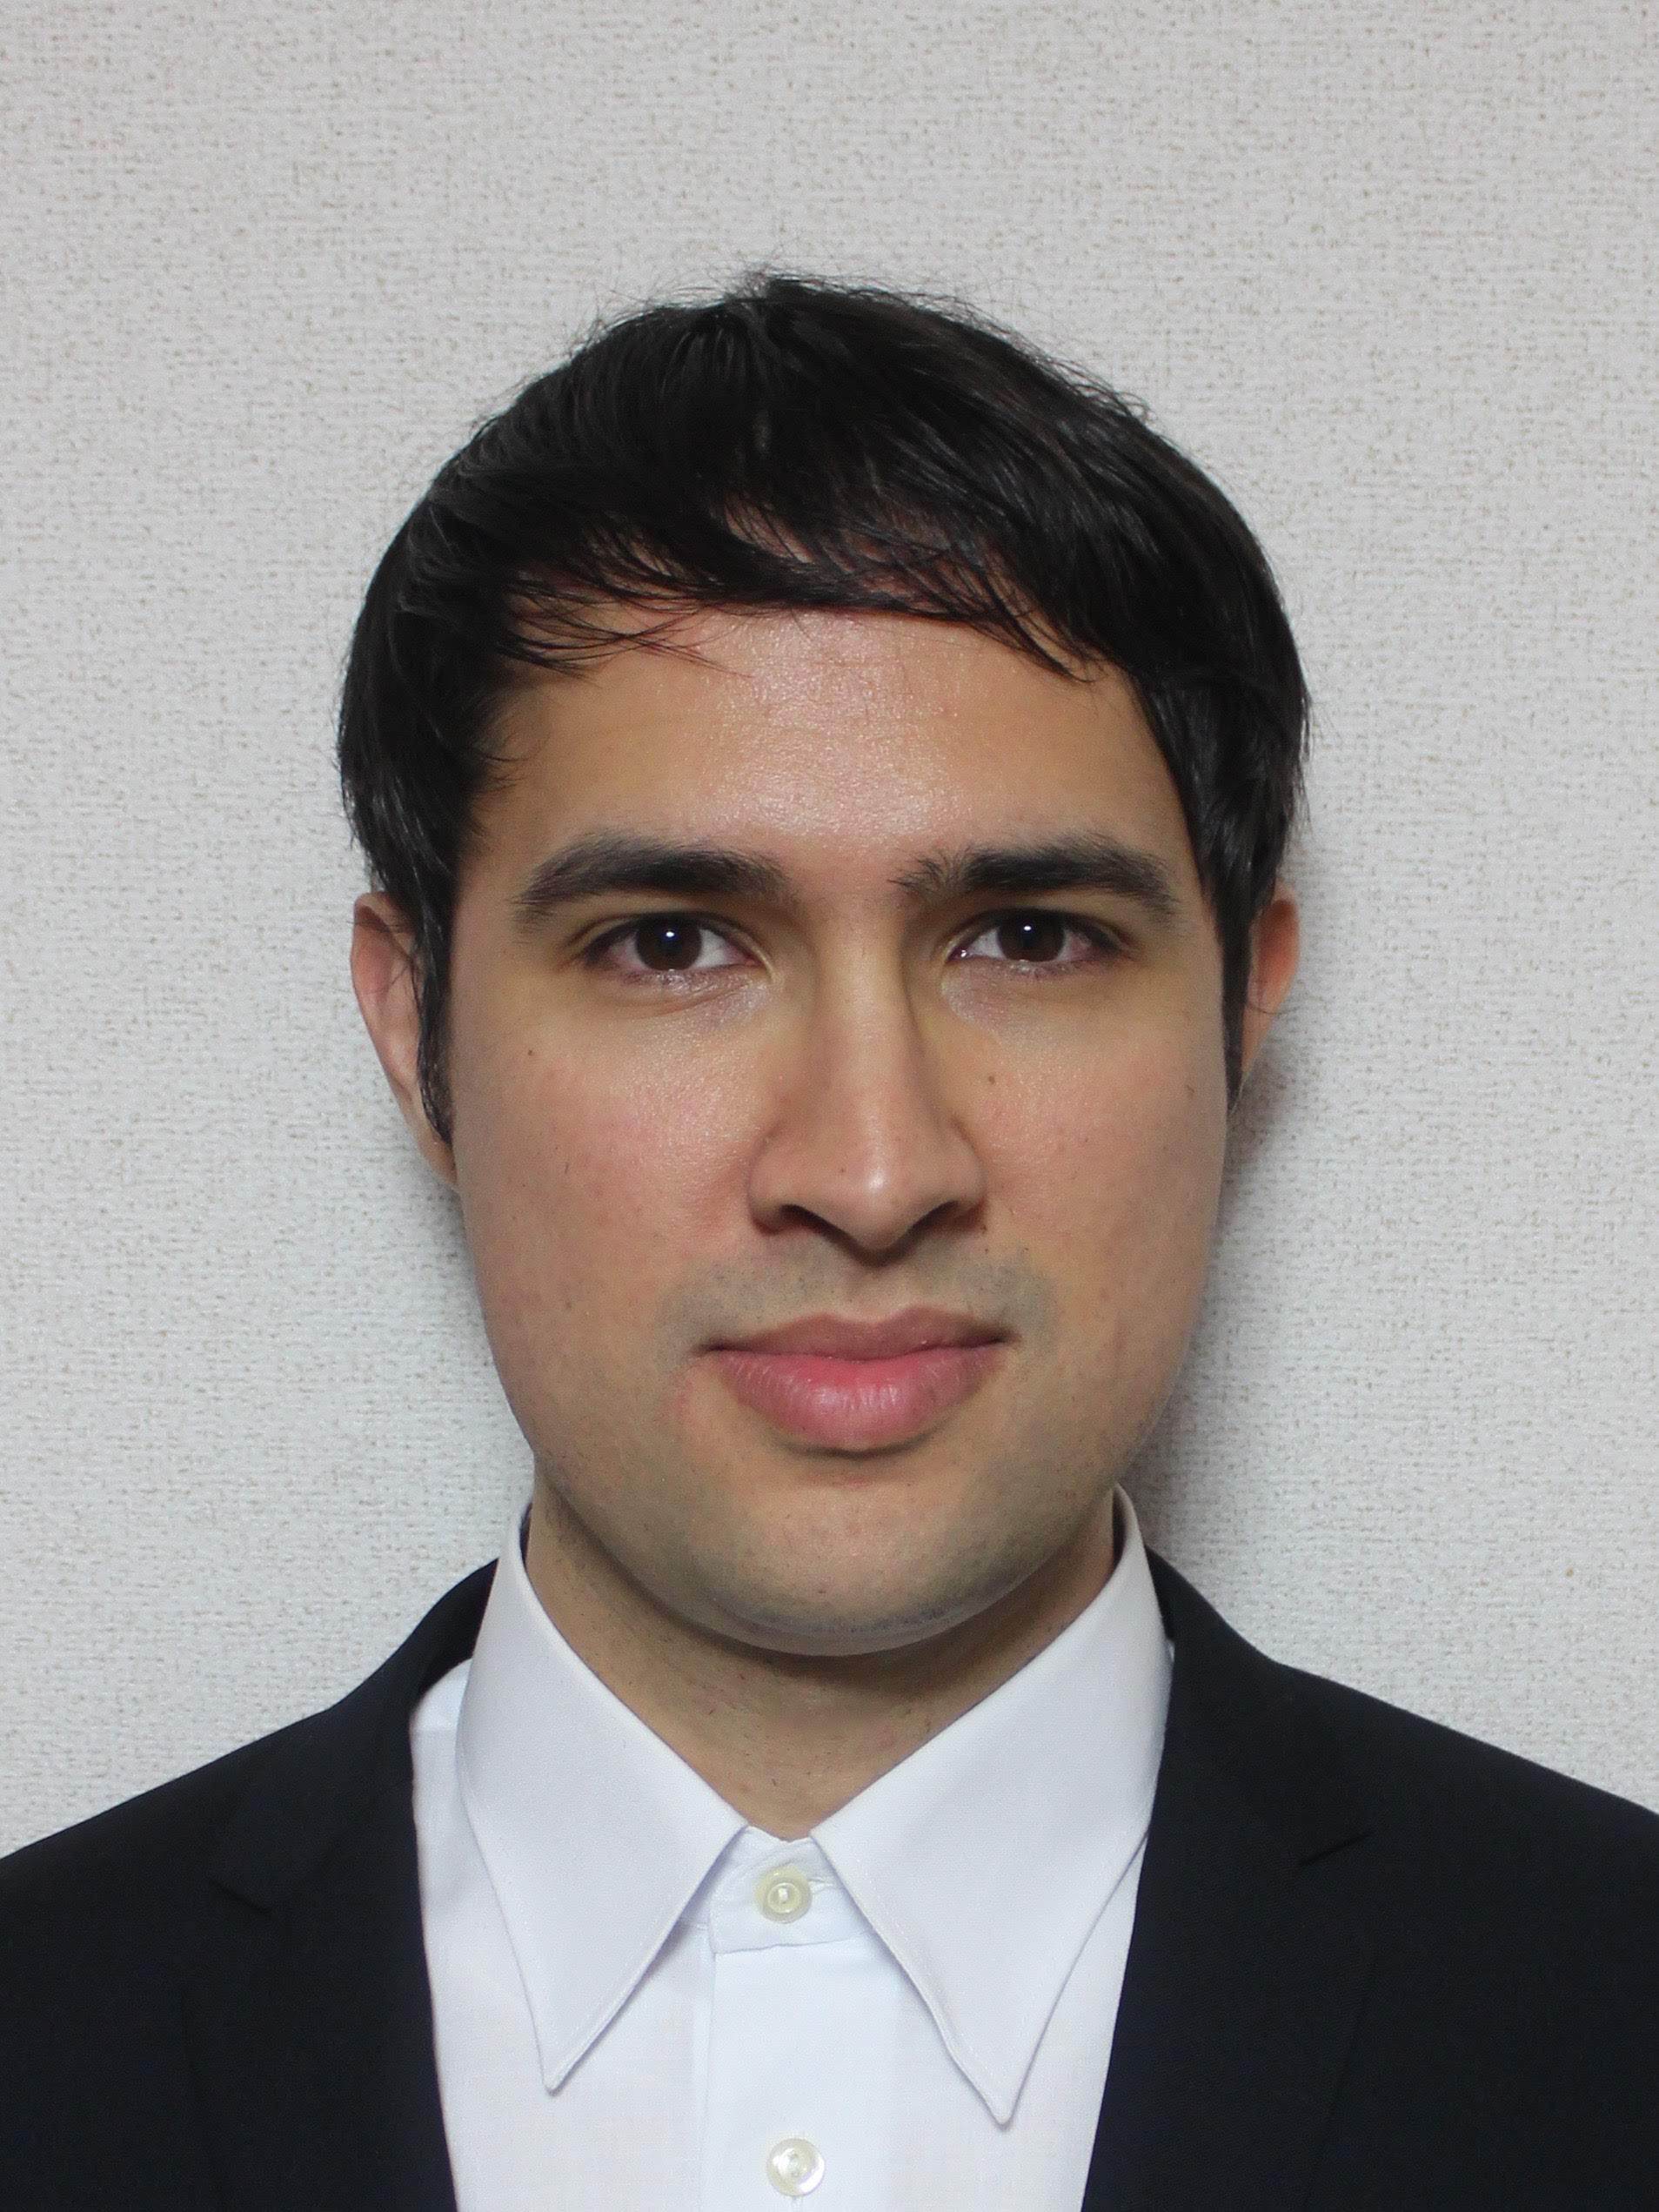
\includegraphics[width=3cm]{data/picture.jpg}}{} \\
    \end{tabularx}
  \end{center}
}

\newcommand{\importdata}{
  \csvnames{publications}{title=\title,year=\year,arxiv=\arxiv,doi=\doi,journal=\journal}
  \csvnames{educations}{degree = \degree,specialization = \specialization,gradyear = \gradyear,entryyear = \entryyear,school = \school,country = \country,city = \city}
  \csvnames{appointments}{position=\position,start_year=\startyear,end_year=\endyear,institution=\institution}
  \csvnames{recommenders}{name=\name,organization=\organization,position=\position,email=\email, relationship=\relation}
  \csvnames{talks}{type=\type,year=\year,month=\month,place=\place,invited=\invited}
  \csvnames{awards}{award=\award,place=\place,year=\year}
  \csvnames{memberships}{organization=\org,start year=\start,end year=\fin,position=\role}
  \csvnames{teaching}{institution=\institution,class=\class,term=\term,note=\note}
}

\newcommand{\employerblurb}[1]{ #1 }
